%pdflatex
\documentclass[12,twoside]{TFG-GCED}
%\usepackage[active]{srcltx}
\usepackage[]{TFG_ARS}
% Body of document

\titol{This is the long title\\[3mm] with a line skip}
\titolcurt{Short title}
\authorStudent{Author's full name}
\supervisors{(name of the supervisor/s of the TFG)\\ Department (or Institution if not UPC)\\ Ponent: nom del ponent si n'hi ha}
\monthYear{Month, year}

%\msc[2010]{Primary  	55M25, 57P10, Secondary 55P15, 57R19, 57N15.}

\paraulesclau{keyword1, keyword2, keyword3, ...}
\agraiments{
Thanks to...}


\abstracteng{This should be an abstract in english, up to 1000 characters.}

%%%%%%%%%
\begin{document}

\maketitle

This is an example of a document using the TFG-GCED.cls document class. The TFG-GCED.cls document class is a modification of the Reports@SCM class with minor differences (cover page, title colors and format for references).

\textbf{Using this template is not mandatory}. Remember that the report should be about 40 pages plus appendices.

In any case, \textbf{you must use the template for the main cover page} \texttt{coverTFG-GCED.doc}. You can follow these steps:
\begin{itemize}
	\item Generate a pdf file with the document of your TFG, following or not this template
	\item Modify the document \texttt{coverTFG-GCED.doc} with the data of your thesis and generate a pdf with two pages (cover and blank page)
	\item Use Adobe or other sofware to join (combine or merge) the two pdf files in one pdf file.
\end{itemize}

\newpage
This report should contain the following information (you can rename the sections):
%This will generate the table of contents:
\continguts


\newpage
\color{black}
\section{Introduction}

The acoustic quality of a space is essential to guarantee an optimal sound expirience. This project aims to develop a Python program capable of analysis acoustic parameters such as frequency response, phase, delay, RT60 and others.

Using a speaker-microphone configuration, the system will allow to automatic correction on the output signal using equalization.

\subsection{Prueba 1}
\subsubsection{Otra Prueba}

\section{State of the art}

\section{Goals of the project}

Develop a system for analysis and measuring acoustic parameters.

Implement an acoustic correction algorithm using equalization.

\section{Proposed solution / Tasks}

\subsection{Review basic concepts of acoustics analysis and correction}

\subsection{Implementation of acoustic analysis}

\subsection{Implementation of acoustic correction}

\subsection{Integration of a monitoring mechanism}

\subsection{Validation and testing of the system}

\section{Results}

\section{Conclusions}

\section*{Bibliography}

See comments below
\section*{Appendix}

See comments below



%%%%
%%%%%
\section*{Comments on Figures}

Please include figures using the graphics package uploaded.  Fancy options can be found for example in  \begin{verbatim} http://www.kwasan.kyoto-u.ac.jp/solarb6/usinggraphicx.pdf \end{verbatim}

\begin{figure}[htb!]
\begin{center}
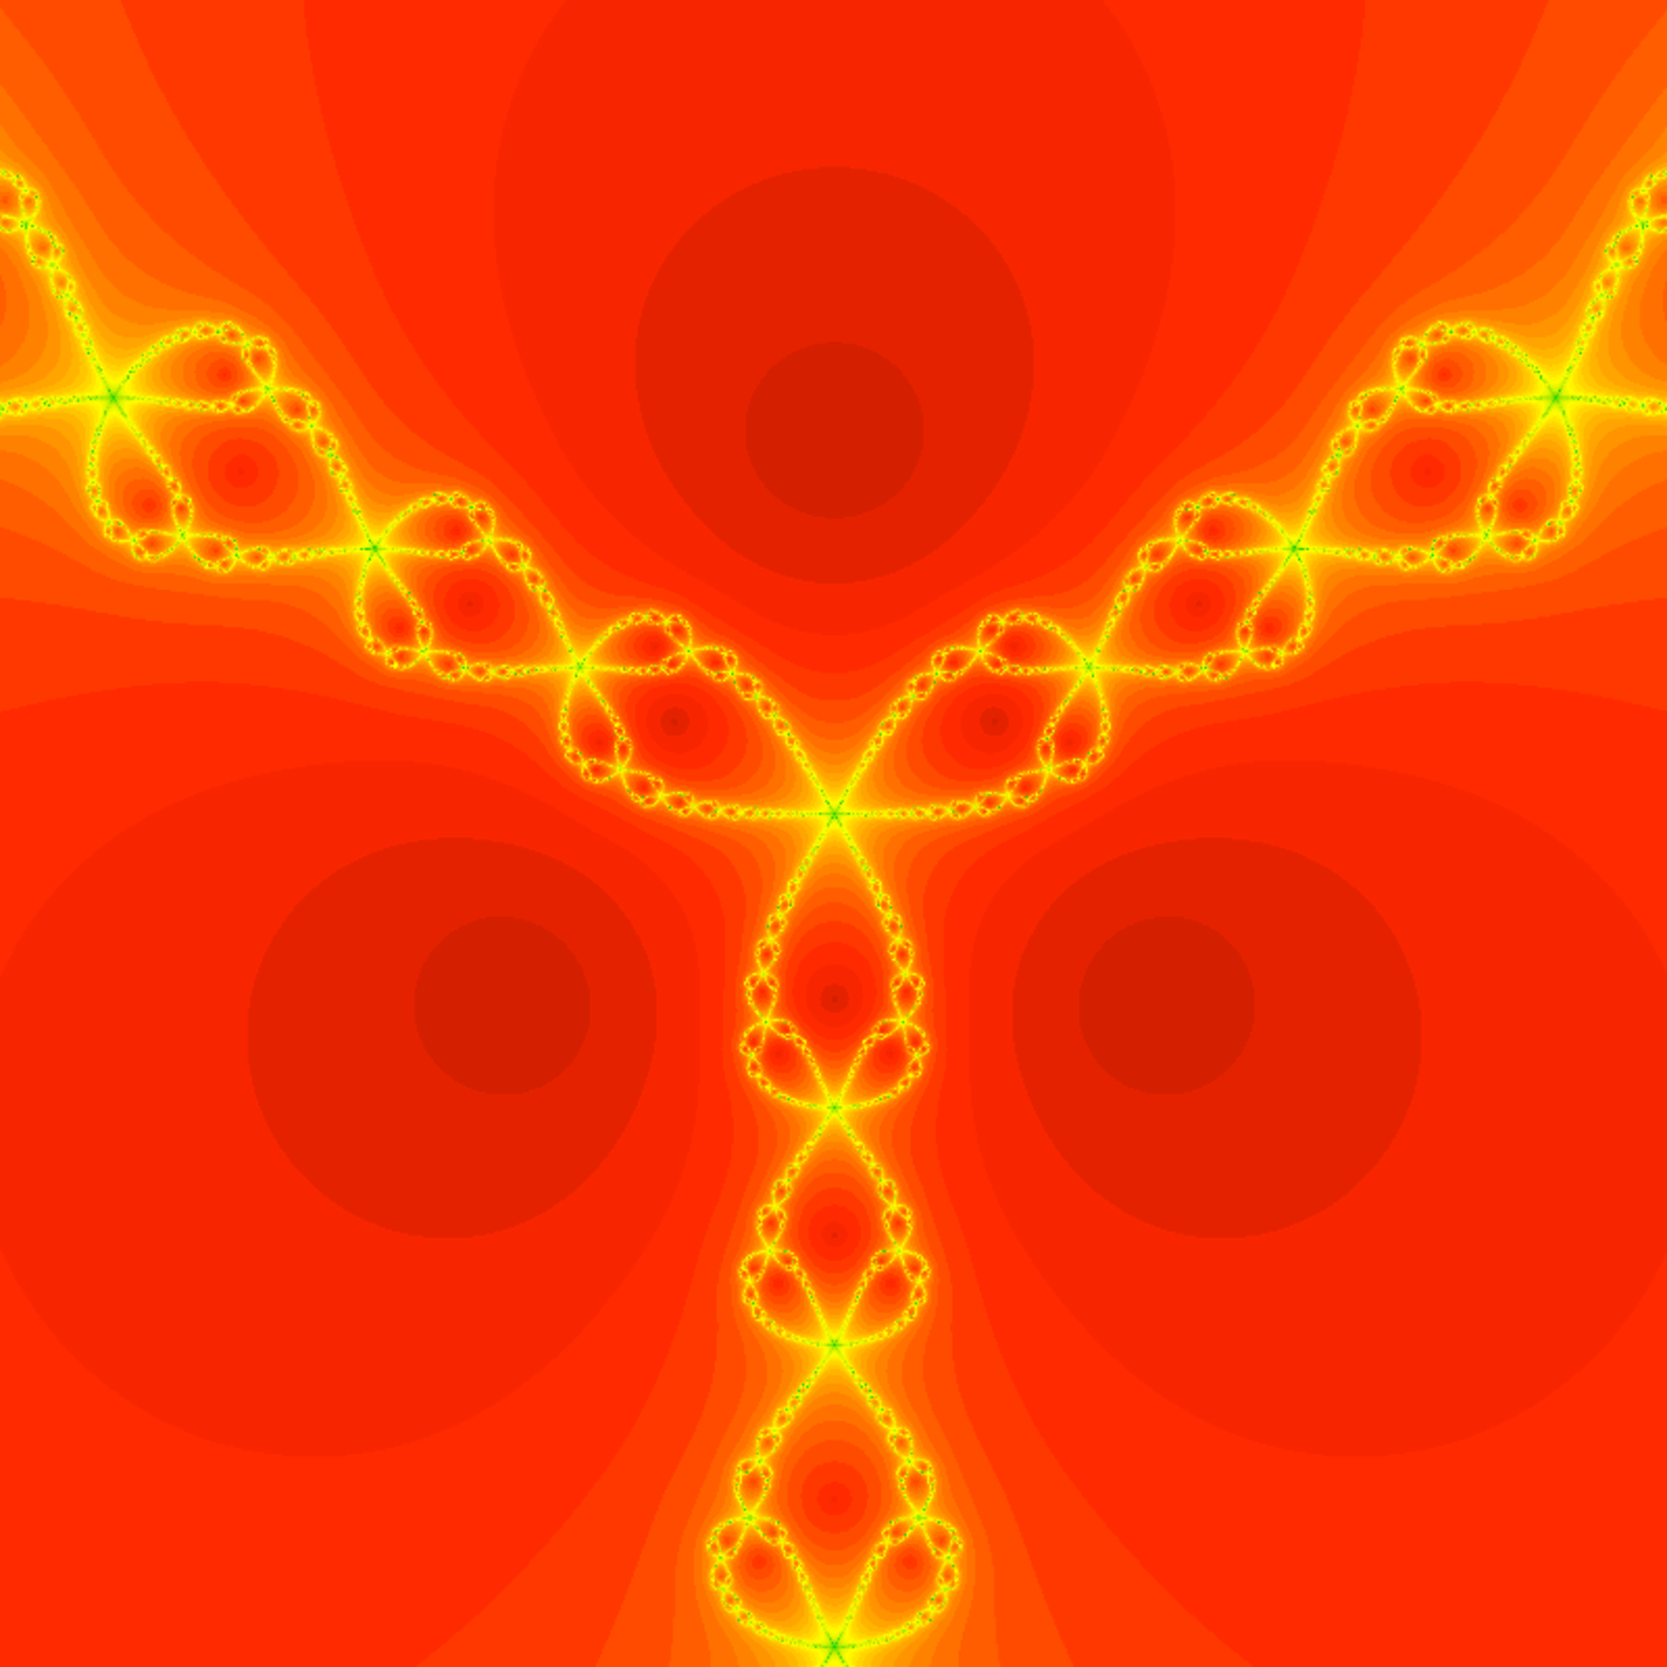
\includegraphics[width=6cm]{samplefigure.pdf}
\end{center}
\caption{\label{sample figure} \small The caption of this figure is ``Newton's method of a cubic polynomial".}
\end{figure}

%%%%%%%%
\section*{ Comments on Mathematics and packages} \label{packages}

By default, the following packages are uploaded:
\begin{enumerate}[\bf (1)]
\item {\tt enumerate:} It allows you to make list with specific somehow arbitrary labels, like this one.
\item {\tt amsthm:} To make evironments with different styles.
\item {\tt amsmath,amssymb,amsfonts:} Multiple mathematics symbols and fonts.
\item {\tt graphicx:} To include figures in a simple and intuitive way.
\item {\tt amscd:} To make commutative diagram with horizontal and vertical arrows. See below.
\item {\tt xy:} To make really fancy commutative arrows. See below.
\item {\tt booktabs:} To make fancy tables.
\end{enumerate}
You may add other standard packages if you need them but try to avoid it if at all possible.

If you need to use them, you will find information about these packages in the usual internet places.

You can use the enviroments defined above:
\begin{theorem} This is my theorem.
\end{theorem}

\section*{Comments on Bibliography}

You may include\cite{ex} your references by hand using {\tt the bibliography} (see an example below) or, alternatively, you may use a .bib file and use BibTeX. In any case, we ask \cite{Mueller2002TransferFunctionMW, ex}you to use a reasonable {\bf consistent} format for all your references. Our recommendation is using BibTex with the style   "plain" or "amsalpha".

%\newpage

\bibliographystyle{amsalpha}
\bibliography{TFG_ARS}

%______________________________________________________________
\appendix
\vfill\newpage \section{Title of the appendix}
You can include here an appendix with details that can not be included in the core of the document. You should reference the sections in this appendix in the core document.
\vfill\newpage \section{Title of the appendix}
Second appendix.

\end{document}


